\documentclass[10pt,twoside]{estiloUBI}




%%%%%%%%%%%%%%%%%%%%%%%%%%%%%%%%%%%%%%%%%%%%%%%%%%%%%%%%%%%%%%%%%%%%%%%%%%%%%%%%%%%%%%%%%%%%%%%%%%%%%%%%%%%%%%
%% Este é o ficheiro formatacaoUBI.tex - NÃO EDITAR excepto a secção hypersetup!
%% Define a formatação a ser usada em teses apresentadadas na Universidade da Beira Interior, seguindo o despacho Reitoral nº 49/R/2010
%% Versão 2.2 - 01/06/2016 - Podem aparecer as palavras "Figura" e "Tabela" nas respectivas listas
%% Versão 2.1 - 28/03/2014 - Agora compila com o XeLaTeX por causa do tipo de fonte, incluido o estilo de biblipgrafia IEEE, possibilidade de escolha de tipo de fonte matemático
%% Versão 2.0 - 10/11/2011 - Bibliografia agora aparece no índice
%% Versão 1.9 - 10/10/2011 - Resolvido problema em que o texto nas tabelas aparecia em cima da linha superior
%% Versão 1.8 - 12/07/2011 - Legendas são agora centradas
%% Versão 1.7 - 8/07/2011 - Correcção de algumas medidas de acordo com novo modelo de Word
%% Versão 1.6 - 1/07/2011 - Trebuchet inserido como fonte principal
%% Adaptado do original de Oliver Commowick para estar de acordo com as regras do Despacho nº 49/R/2010
%% Adaptação por João Ferro, Norberto Barroca, Luís Borges, Rui Paulo, Aleksandra Nadziejko - Instituto de Telecomunicações - DEM/UBI, Paulo Machado - Departamento de Ciências Aeroespaciais/UBI.
%% Contacto: latex@e-projects.ubi.pt
%% Agradecimento especial a Stefan_K da latex-community.org pela ajuda com os códigos de tabela e equação.
%% A versão actual pode ser alterada sem aviso prévio.
%% Download da última versão em área reservada: http://www.UBI.pt
%% Uso e distribuição de acordo com a licenca GNU GPL.
%% 
%%    Este programa é um software livre: você pode redistribui-lo e/ou 
%%
%%		modificá-lo dentro dos termos da Licença Pública Geral GNU como 
%%
%%		publicada pela Free Software Foundation, na versão 3 da 
%%
%%		Licença, ou (na sua opinião) qualquer versão.
%%
%%
%%
%%		Este programa é distribuido na esperança que possa ser útil, 
%%
%%		mas SEM NENHUMA GARANTIA; sem uma garantia implícita de ADEQUAÇÃO a qualquer
%%
%%		MERCADO ou APLICAÇÃO EM PARTICULAR. Veja a
%%
%%		Licença Pública Geral GNU para maiores detalhes.
%%
%%
%%
%%		Você deve ter recebido uma cópia da Licença Pública Geral GNU
%%
%%		junto com este programa, se não, veja <http://www.gnu.org/licenses/>.
%%%%%%%%%%%%%%%%%%%%%%%%%%%%%%%%%%%%%%%%%%%%%%%%%%%%%%%%%%%%%%%%%%%%%%%%%%%%%%%%%%%%%%%%%%%%%%%%%%%%%%%%%%%%%%


% Pacotes a incluir
\usepackage{mathspec}
\usepackage{fontspec}
\usepackage{amsmath,amscd,amsthm,xspace}	%Pacotes matemáticos 
\usepackage{amssymb}						%Fontes extra para matemáticos   http://www.ctan.org/tex-archive/fonts/amsfonts
%\usepackage[math]{kurier} %descomentar para colocar tipo de letra aproximado ao Trebuchet nos ambientes matemáticos

%\usepackage[latin1]{inputenc}		%este faz falta na versão normal, mas em XeLaTeX tem que ser comentado		%Permitir caracteres acentuados  http://www.ctan.org/pkg/inputenc
%\usepackage[T1]{fontenc}					%este faz falta na versão normal, mas em XeLaTeX tem que ser comentado		%Permitir caracteresespeciais  http://www.ctan.org/pkg/fontenc

\usepackage[a4paper,left=3.5cm,right=2.5cm,top=2.5cm,bottom=2.5cm]{geometry}	%Papel A4, com margens
%\renewcommand{\baselinestretch}{1.05}

\usepackage{aecompl}								%Permitir fontes vituais para codificação T1  http://www.ctan.org/tex-archive/fonts/ae
\usepackage[center,nooneline,font={footnotesize}]{caption}			%Legenda: centrada, tamanho de nota rodapé  http://www.ctan.org/pkg/caption
\setlength{\parindent}{0pt}							%Sem tabulação em cada novo parágrafo
%\usepackage{parskip}								%Layout with zero \parindent, non-zero \parskip http://www.ctan.org/pkg/parskip
%\setlength{\parskip}{0.53cm}



%% O código seguinte permite gerar um mini indice de capitulo (não referido no despacho reitoral)
% \usepackage[nottoc, notlof, notlot]{tocbibind}
% \usepackage{minitoc}
% \setcounter{minitocdepth}{2}
% \mtcindent=15pt
%%Usar \minitoc para colocar o mini indice de capitulo


%% Verificar se saída é pdf directo e ajustar o formato imagens a isso
%\usepackage{ifpdf}
%\ifpdf
%  \usepackage[pdftex]{graphicx}							%Inserir gráficos  http://ctan.org/pkg/graphicx
\usepackage{graphicx}
%    \DeclareGraphicsExtensions{.jpg,.png} 					%Pdf directo apenas compativel com jpg, png...
  \usepackage[pagebackref,hyperindex=true]{hyperref}				%O pacote hyperref é usada para lidar com comandos referência cruzada  http://ctan.org/pkg/hyperref
%\else
%  \usepackage{graphicx}
%  \DeclareGraphicsExtensions{.ps,.eps}						%DVI directo apenas compativel com ps, eps...
%  \usepackage[dvipdfm,pagebackref,hyperindex=true]{hyperref}
%\fi


\graphicspath{{.}{imagens/}}							%Directorio das imagens


%%Links do pdf
\usepackage{color}								%Pacote de gestão de cor
\definecolor{linkcol}{rgb}{0,0,0} 						%Cor das hiperligações (preto)
\definecolor{citecol}{rgb}{0,0,0} 						%Cor das referências à bibliografia no texto (preto)


%% O código seguinte será incluído no pdf gerado http://www.tug.org/applications/hyperref/manual.html
%%Visto nas propriedades do documento
% \hypersetup
% {
% bookmarksopen=true,
% pdftitle="Tese",		%Título
% pdfauthor="João", 		%Autor
% pdfsubject="Tese", 		%Assunto
% pdfmenubar=true,		%Mostrar barra menus
% pdfhighlight=/O, 		%Efeito ao clicar link
% colorlinks=true, 		%Cor em hiperligações
% pdfpagemode=UseNone, 		%Nenhum modo de páginas
% pdfpagelayout=SinglePage, 	%Abertura em modo de página simples
% pdffitwindow=true, 		%Adaptar página à janela
% linkcolor=linkcol, 		%Cor das ligações internas do documento
% citecolor=citecol, 		%Cor das referências à bibliografia no texto
% urlcolor=linkcol 		%Cor das hiperligações
% }


%%Definições variadas
\setcounter{secnumdepth}{3}
\setcounter{tocdepth}{2}


%%Comandos e atalhos para algumas funções matemáticas
\newcommand{\pd}[2]{\frac{\partial #1}{\partial #2}}
\def\abs{\operatorname{abs}}
\def\argmax{\operatornamewithlimits{arg\,max}}
\def\argmin{\operatornamewithlimits{arg\,min}}
\def\diag{\operatorname{Diag}}
\newcommand{\eqRef}[1]{(\ref{#1})}


%%Para rotação de figuras e tabelas http://www.ctan.org/tex-archive/macros/latex/contrib/rotating
 \usepackage{rotating}
  
	
%%Cabeçalho e rodapé http://www.ctan.org/tex-archive/macros/latex/contrib/fancyhdr
\usepackage{fancyhdr}                   						%Fancy Header and Footer
\pagestyle{fancy}                      							%Cabeçalho e rodapé estilo fancy
\fancyfoot{}                            						%Apaga rodapé actual
\fancyhead{}										%Apaga cabeçalho actual
\fancyfoot[LE,RO]{\thepage}   								%Número de paginas no exterior L=left, E=even, R=right, O=Odd
\newcommand{\cabecalho}[1]{\fancyhead[RE,LO]{\bfseries{#1}}}				%Nome da tese no cabeçalho
\let\headruleORIG\headrule
\renewcommand{\headrule}{\color{black} \headruleORIG}
\renewcommand{\headrulewidth}{0pt}							%Régua para cabecalho, 0pt=off, 1pt=on


%Formatação dos tipos de letra
\newcommand{\capitulos}{\fontsize{22pt}{10pt}\bfseries\selectfont}			%Capítulo: 22pt, negrito
\newcommand{\titulos}{\fontsize{18pt}{10pt}\bfseries\selectfont}			%Titulos: 18pt, negrito
\newcommand{\seccao}{\fontsize{14pt}{20pt}\bfseries\selectfont}				%Secção: 14pt, negrito
\newcommand{\subseccao}{\fontsize{12pt}{14pt}\selectfont}				%subsecção: 12pt, normal
\renewcommand{\footnotesize}{\fontsize{9pt}{12pt}\selectfont}				%Nota rodapé: 9pt, espacamento 1 linha
\renewcommand{\Huge}{\titulos}


%Folha de rosto
\newcommand{\rostoubi}{\fontsize{14pt}{14pt}\selectfont}				%Texto a dizer UBI 14pt, normal
\newcommand{\rostotitulo}{\fontsize{18pt}{18pt}\selectfont}				%Titulo da tese: 18pt, (+negrito)
\newcommand{\rostosubtit}{\fontsize{16pt}{16pt}\selectfont}				%Titulo da tese: 16pt, (+negrito)
\newcommand{\rostonomes}{\fontsize{14pt}{14pt}\selectfont}				%Nome autor, curso: 14pt, (+negrito)
\newcommand{\rostooutros}{\fontsize{12pt}{12pt}\selectfont}				%Local e data: 12pt, (+negrito)
\newcommand{\rostofac}{\fontsize{12.5pt}{12.5pt}\selectfont}				%Faculdade: 12.5pt




%%Passar para português
%\newcommand{\portugues}{\usepackage[portuguese]{babel}		%Descomentar para escrever com regras em Português sem ser em XeLaTeX  http://www.ctan.org/pkg/babel  								% Users of X∃TeX are ad­vised to use poly­glos­sia rather than Ba­bel.

\newcommand{\portugues}{\usepackage{polyglossia} %Comentar para escrever sem ser em modo XeLaTeX http://www.ctan.org/tex-archive/macros/latex/contrib/polyglossia
\setmainlanguage{portuges}                       %Comentar para escrever sem ser em modo XeLaTeX

\addto\captionsportuguese{\renewcommand{\contentsname}{Índice}}
\addto\captionsportuguese{\renewcommand{\indexname}{Índice Remissivo}}}

%linhas das tabelas e afins
\usepackage{colortbl}									%Adicionar cor às tabelas  http://www.ctan.org/tex-archive/macros/latex/contrib/colortbl/
\arrayrulecolor{black}									%Preto


%Estilo plain modificado
\fancypagestyle{plain}{
  %\fancyhead{}	
  %\fancyfoot{}
  \renewcommand{\headrulewidth}{0pt}
}


%%Para algoritmos  http://www.ctan.org/tex-archive/macros/latex/contrib/algorithms/
\usepackage{algorithm}
\usepackage[noend]{algorithmic}


%%Páginas em branco geradas antes de capítulos têm de vir numeradas
\makeatletter

\def\cleardoublepage{\clearpage\if@twoside \ifodd\c@page\else%
  \hbox{}%
  \thispagestyle{plain}%              							%Páginas em branco usam estilo plain
  \newpage%
  \if@twocolumn\hbox{}\newpage\fi\fi\fi}

\makeatother


%%Tabela com 9pt
%\makeatletter										%O código comentado apresentado apresenta problemas
%\renewenvironment{table}{%								%Procurar no forum http://latex-community.org, tópico "Equation Numbering and Table Font Size''
  %\@float{table}\footnotesize}
  %{\end@float}
%\makeatother
\usepackage{etoolbox}									%Para modificar o tamanho de letra na tabela http://ctan.org/pkg/etoolbox
\AtBeginEnvironment{tabular}{\footnotesize}						%Procurar no forum http://latex-community.org, tópico "Equation Numbering and Table Font Size''


%%Número de equação centrado com equação
\makeatletter										%Explicação  http://tex.stackexchange.com/questions/8351/what-do-makeatletter-and-makeatother-do
\def\place@tag{\quad\boxz@}								%Comentar esta linha para alinhar número da equação à direita
\makeatother
\let\equation\align
\let\endequation\endalign
 

%%Código herdado
\newenvironment{maxime}[1]
{
\vspace*{0cm}
\hfill
\begin{minipage}{0.5\textwidth}%
%\rule[0.5ex]{\textwidth}{0.1mm}\\%
\hrulefill $\:$ {\bf #1}\\
%\vspace*{-0.25cm}
\it 
}%
{%

\hrulefill
\vspace*{0.5cm}%
\end{minipage}
}

%mninitoc
%\let\minitocORIG\minitoc
%\renewcommand{\minitoc}{\minitocORIG \vspace{1.5em}}

\usepackage{multirow}					%Create tab­u­lar cells http://www.ctan.org/tex-archive/macros/latex/contrib/multirow
% \usepackage{slashbox}					%Pro­duce tab­u­lar cells with di­ag­o­nal lines in them http://www.ctan.org/pkg/slashbox

\newenvironment{bulletList}				%http://en.wikibooks.org/wiki/LaTeX/List_Structures
{ \begin{list}%
	{$\bullet$}%
	{\setlength{\labelwidth}{25pt}%
	 \setlength{\leftmargin}{30pt}%
	 \setlength{\itemsep}{\parsep}}}%
{ \end{list} }

\newtheorem{definition}{Définition}
\renewcommand{\epsilon}{\varepsilon}

% centered page environment

\newenvironment{vcenterpage}
%{\newpage\vspace*{\fill}\fancyhf{}\renewcommand{\headrulewidth}{0pt}}
{\newpage\vspace*{\fill}\renewcommand{\headrulewidth}{0pt}}
{\vspace*{\fill}\par\pagebreak}

\usepackage{setspace}					%Pro­vides sup­port for set­ting the spac­ing be­tween lines http://www.ctan.org/tex-archive/macros/latex/contrib/setspace
\usepackage{tabularx}					%The pack­age de­fines an en­vi­ron­ment tab­u­larx, an ex­ten­sion of tab­u­lar  http://www.ctan.org/pkg/tabularx
\usepackage{makeidx}					%Index processor  http://www.ctan.org/tex-archive/indexing/makeindex
\newcolumntype{Y}{>{\raggedright\arraybackslash}X}

%% Inicio do bloco
%% Descomentando o este bloco de comandos as  palavras "Figura" e "Tabelas" vão aparecer por extenso nas respectivas Listas
%%
%% Comentado aparece:
%%Lista de Figuras
%%		2.1 Circuito básico com uma fonte de tensão contínua (V) e uma resistência atraves-
%%			sada por uma corrente I. . . . . . . . . . . . . . . . . . . . . . . . . . . . . .3
%%
%% Descomentando aparece
%% 		Figura 2.1 Circuito básico com uma fonte de tensão contínua (V) e uma resistência
%%      atravessada por uma corrente I. . . . . . . . . . . . . . . . . . . . . .3
%%
%\usepackage[titles]{tocloft}
%\newlength{\mylen}
%
%\renewcommand{\cftfigpresnum}{\figurename\enspace}
%\renewcommand{\cftfigaftersnum}{ }
%\settowidth{\mylen}{\cftfigpresnum\cftfigaftersnum}
%\addtolength{\cftfignumwidth}{\mylen}
%
%\renewcommand{\cfttabpresnum}{\tablename\enspace}
%\renewcommand{\cfttabaftersnum}{ }
%\settowidth{\mylen}{\cfttabpresnum\cfttabaftersnum}
%\addtolength{\cfttabnumwidth}{\mylen}
%% Fim do Bloco


\usepackage{fontspec}


%%Comentar a linha seguinte se escrever a tese em inglês
\portugues


%%Para índice remissivo
\makeindex


%%Escolher tipo de letra a usar:
%\usepackage{lmodern}												%Latin modern
%\usepackage{palatino}												%Palatino
%\usepackage{times}												    %Times


%%O comando seguinte insere o nome da tese no cabeçalho das páginas (comentar se não for pretendido)
\cabecalho{Moeda Criptográfica Controlada Centralmente}



\begin{document}

%%O comando seguinte insere o espaçamento de 1.5 linhas
\onehalfspacing

%%Página de rosto
\pagenumbering{roman}


%\dominitoc


%%Numeração das páginas
\pagestyle{fancy}


%%O comando a seguir gera uma página após a de rosto com cabeçalho e rodapé
% \cleardoublepage

%%O comando a seguir permite que as costas da página de rosto não inclua cabeçalho mas rodapé (escolher entre este e outro)
%\newpage\mbox{}\thispagestyle{plain}\fancyhead{}


%%Dedicatória

%\newpage 	
%\mbox{}
%\vfil
%\begin{center}
%Dedicated to...
%\end{center}
%\vfil
%\eject
%\cleardoublepage


%%Agradecimentos 



%%Prefácio 



%%Resumo+palavras-chave


%%Resumo alargado 


%%abstract+keywords


%%Índice

%%Lista de figuras
{\begin{titlepage}
\begin{center}

\begin{flushleft}
 
\includegraphics[height=2.22cm]{logo}\\
\rostoubi UNIVERSIDADE DA BEIRA INTERIOR\\
\rostofac Engenharia\\
\end{flushleft}

\vspace{5.6cm}

\rostotitulo \textbf{ Moeda Criptográfica Controlada Centralmente} \\
\rostosubtit \textbf{Fr€coin}\\

\vspace{1.8cm}

\rostonomes \textbf{Guilherme Calado Boino, M8468\\
João Alexandre de Aguiar Amaral dos Santos, M8810 \\
Nelson Ricardo Matos Fonseca, M8351\\
Vasco Ferrinho Lopes, M8486}\\

\vspace{1.4cm}

\rostooutros Trabalho Prático Sistemas Software Seguros\\
\rostonomes \textbf{Engenharia Informática}\\
\rostooutros (2º ciclo de estudos)\\

\vspace{3.3cm}

\rostooutros Orientador: Prof. Doutor Pedro Ricardo Morais Inácio\\
%Co-orientador: Prof. Doutor Nome\\

\vspace{1.4cm}

\rostooutros \textbf{Covilhã, Maio de 2018}

\end{center}
\end{titlepage}

 \let\cleardoublepage\clearpage}


\newpage \let\cleardoublepage\clearpage
\section*{\titulos{Resumo}}
Com o aparecimento e crescimento que tecnologias como a Bitcoin tiveram nos últimos anos, e devido às suas características criptgráficas, torna-se interessante abordar a sua constituição. Assim, introduzimos a Fr€€Coin, uma moeda criptográfica controlada centralmente.
A Fr€€Coin baseia-se num sistema central de confiança que controla a quantidade existente da moeda e todas as transações, além de controlar a atribuição de moedas a partir de desafios feitos aos utilizadores, de dificuldade variável.

!!!!!!!!!!!!!!!!!!!!!!!!!!!!!!!!


{\tableofcontents \let\cleardoublepage\clearpage
\listoffigures \let\cleardoublepage\clearpage
\listoftables \let\cleardoublepage\clearpage}

% \cleardoublepage


%%Abreviaturas
\newpage \let\cleardoublepage\clearpage
\section*{\titulos{Lista de Acrónimos}}
\vspace{0.5cm}
  \begin{tabularx}{\linewidth}{c p{0.5cm} Y}
 	UBI & & Universidade da Beira Interior\cr
 	MPSOCD & & Multi-objective Particle Swarm Optimization Crowding Distance
 	\end{tabularx}
%  \cleardoublepage
  

%% Os capitulos são inseridos a partir daqui 
 
\mainmatter

{\chapter{Introdução}
\label{chap:int}

%% Para fazer um mini indice do capitulo abrir o ficheiro ``formatacaoUBI.tex" e procurar ''%% O código seguinte permite gerar um mini indice de capitulo (não referido no despacho reitoral)''
%\minitoc


\section{Descrição do Problema}
Com cada vez mais o uso das novas tecnologias, cada vez mais existe a necessidade da existência de moedas criptográficas. Para a cria uma moeda eletrónica, todas as comunicações devem ser cifradas com chaves públicas e privadas de forma a manter a autenticidade do utilizador, para que a troca de mensagens seja segura. Por outro lado, para a criação da moeda existem tarefas que são enviadas por parte do utilizador onde o utilizador que resolver esse problema irá ser compensado. Os utilizadores, podem ainda efetuar transações entre eles sempre com o conhecimento do servidor que controla todo o dinheiro eletrónico que existe no sistema e em cada utilizador.


A aplicação, fornece assim mecanismos para a criação de um utilizador com a criação das suas chaves publica e privada e todas as mensagens são então cifradas com as chaves (tanto do servidor como do utilizador), o que faz com que haja autenticidade de ambas as partes. A aplicação é capaz de enviar com um tempo definido as tarefas a serem tratadas pelos utilizadores e receber as suas respostas de forma a outros utilizadores poderem parar de executar essa tarefa.


\section{Constituição do Grupo}
O grupo é constituído pelos seguintes discentes de Mestrado de Engenharia Informática da Universidade da Beira Interior, sendo estes:

\begin{itemize}
    \item Guilherme Calado Boino-M8468
    
    \item João Alexandre de Aguiar Amaral dos Santos-M8810
    
    \item Nelson Ricardo Matos Fonseca-M8351
    
    \item Vasco Ferrinho Lopes-M8486
    
\end{itemize}




\section{Organização do Documento}

De modo a refletir o trabalho que foi feito, este documento encontra-se estruturado da seguinte forma:
\begin{enumerate}
    %\item O primeiro capítulo -- \textbf{Resumo} -- faz uma breve descrição dos objetivos do trabalho, bem como a abordagem tomada para alcançar os mesmos.
    \item O primeiro capítulo -- \textbf{Introdução} -- descreve o problema e a constituição do grupo, bem como a organização do documento.
    
    \item O segundo capítulo -- \textbf{Engenharia de Software e da Segurança} -- faz uma análise crítica aos requisitos e aos caos de uso, bem como uma abordagem ao modelos do sistema e dos ataques que podem ou não ser efetuados.
    
    \item O terceiro capítulo -- \textbf{Implementação} -- aqui são descritos detalhes técnicos acerca da implementação de código, algoritmos utilizados e manuais de instalação e configuração.
   
    \item O quarto capítulo -- \textbf{Testes ao Sistema} -- enumera os testes de segurança e dos resultados obtidos para os testes realizados.
    
    \item O quinto capítulo -- \textbf{Reflexão Crítica e Problemas Encontrados} -- enumera os objetivos alcançados, bem como os problemas encontrados e a divisão de tarefas efetuada.
    
    \item O sexto capítulo -- \textbf{Conclusões e Trabalho Futuro} -- são tiradas as ilações finais acerca de todo o desenvolvimento do projeto.
\end{enumerate} \let\cleardoublepage\clearpage
% \cleardoublepage
\chapter{Engenharia de Software e da Segurança}
\label{chap:engsoft}

\section{Análise dos Requisitos e Casos de Uso}
\label{sec:analreq}
De forma ao sistema corresponder a todas as expectativas, foi elaborada uma lista de requisitos composta por:

\begin{enumerate}
    \item Deve ser efetuadas comunicações(seguras) cliente-servidor e servidor-cliente.
    
    \item O utilizador deve realizar um registo inicial onde é gerado um par de chaves (pública e privada).
    
    \item O sistema deve permitir transações entre os seus clientes.
    
    \item O sistema deve lançar desafios de forma a criar novas moedas(fr€coin).
    
    \item O sistema deve suportar transações completamente anónimas entre utilizadores.
    
    \item A entidade central é também autoridade certificadora(servidor).
    
    \item O sistema deve ser implementado sobre curvas elípticas.
    
    \item O sistema deve suportar efetuar operações em simultâneo de forma a efetuar trabalho.
    
    \item O sistema deve lançar desafios sobre um tempo pré definido.
    
    \item O sistema deve ser capaz de controlar o número de fr€coin existente.
    
    \item O servidor deve ser uma entidade de confiança.
    
    \item O servidor deve conter informação acerca do nome do utilizador, a sua chave publica !!!!MAIS!!!!.
    
    \item O servidor deve conter todos os documentos das transações assinados pelas entidades que as efetuam.
    
    \item O cliente deve conter o seu par de chaves (pública e privada) e a chave pública do servidor.
    
\end{enumerate}

Quanto aos casos de uso, estes podem ser da forma:
!!!!!!!!!!!!!!!!!!!VERIFICAR DIAGRAMAS E MUDAR, ESTA NO PC BOINO OS DIAGRAMAS!!!!!!!!!!!!!!!!!!!


\begin{figure}[H]
\centering
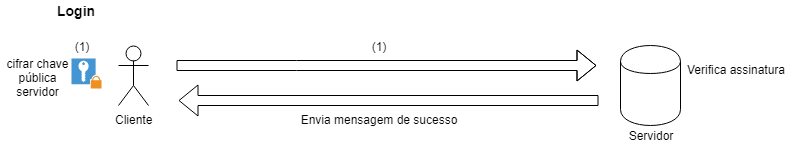
\includegraphics[width=.7\textwidth]{imagens/login.png}
\caption{Diagrama de login.}
\label{fig7}
\end{figure}


Sempre que se efetua o login, o utilizador envia um ficheiro cifrado com a sua chave privada, quando este pacote chega ao utilizador este verifica a assinatura e então é efetuado o login para esse cliente.

\begin{figure}[H]
\centering
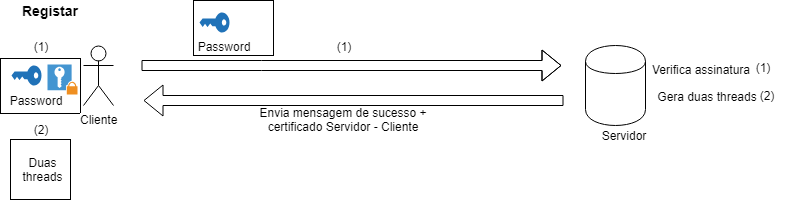
\includegraphics[width=.7\textwidth]{imagens/Registar.png}
\caption{Diagrama de Registar.}
\label{fig7}
\end{figure}


Neste diagrama, podemos verificar que o cliente irá efetuar uma comunicação com o servidor após este enviar uma mensagem encriptada. Ao chegar ao servidor é verificado e guardada o nome do utilizador e a sua chave pública correspondente, desta forma irá enviar uma resposta ao cliente e a partir desse momento podem assim efetuar uma ligação segura.

\begin{figure}[H]
\centering
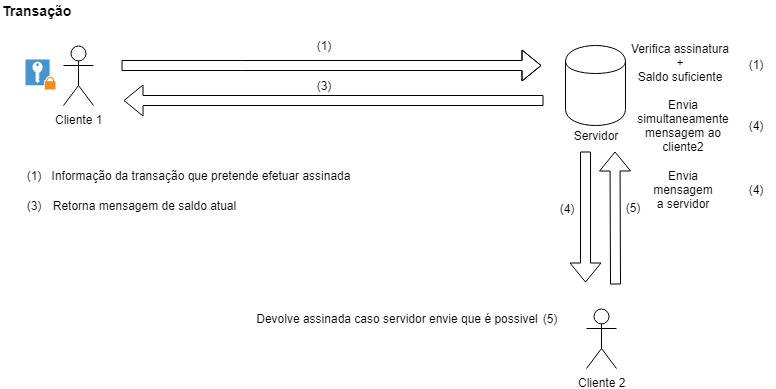
\includegraphics[width=.7\textwidth]{imagens/Transação.png}
\caption{Diagrama de transação.}
\label{fig7}
\end{figure}


Sempre que se pretende efetuar uma transação, o cliente envia uma mensagem ao servidor, assinada com a sua chave privada. Ao chegar ao servidor, este verifica a sua assinatura e se o cliente contem verba suficiente para esta transação. Se o cliente tiver esse montante descrito, é então enviada uma mensagem ao cliente 2(recetor) e é assinado por este. Caso não contenha a verba suficiente o cliente 2 apenas irá verificar a mensagem no entanto não a irá assinar. 
Todas as transações devem passar pelo servidor e com isso serem todas armazenadas no mesmo para mais tarde poderem ser verificadas.


\section{Outros Diagramas}
\label{sec:diagramas}


!!!!!!!!!!FAZER MODELOS DE ATAQUE??????ALGUNS BASICOS??????????!!!!!!!!!!

\section{Modelo do Sistema, Modelos de Ataque e propriedades de Segurança}
\label{sec:modelos}

\section{Modelação de Ataques}
\label{sec:ataques}

\section{Conclusão}
\label{sec:conclusao}

 \let\cleardoublepage\clearpage
\chapter{Implementação}
\label{chap:implmentacao}

\section{Ferramentas e Tecnologias utilizadas}
\label{sec:ferramentas}
O projeto foi desenvolvido de forma a ser usado num computador, para tal foi utilizada a linguagem \textit{Java}, compilada e testada no IDE \textit{NetBeans}. De forma a se encontrar disponível para todos os discentes podendo trabalhar em simultâneo e efetuando controlo de versões.


Desta forma, resulta uma aplicação que corre em linha de comandos (CLI) e um relatório concebido em \emph{Share} \LaTeX



\section{Escolhas de Implementação}
\label{sec:escolhas}

Numa fase inicial, foi necessário tomar algumas decisões fulcrais. Algumas destas decisões basearam-se na escolha da linguagem a ser usada, desta forma foi escolhida a linguagem \textit{Java} derivado a ser uma linguagem orienteada a objetos e também com a criação de uma interface CLI.

\section{Detalhes de Implementação}
\label{sec:detalhes}

\section{Manual de Instalação}
\label{sec:instalacao}

\section{Manual de Utilização}
\label{sec:utilizacao}

\section{Conclusão}
\label{sec:conc} \let\cleardoublepage\clearpage
\chapter{Testes ao Sistema}
\label{chap:testes}

\section{Testes de Segurança}
\label{sec:seguranca}

\section{Resultados}
\label{sec:resultados}

\section{Conclusão}
\label{sec:conclusTestes} \let\cleardoublepage\clearpage
\chapter{Reflexão Crítica e Problemas Encontrados}
\label{chap:reflexao}

\section{Objetivos Propostos vs Alcançados}
\label{sec:objetivos}
O principal objetivo deste trabalho prático foi a elaboração de um programa em CLI onde fosse permitida a ligação através de um par de chaves pública e privada para que dessa forma seja efetuadas conceções para uma prova de trabalho (desta forma podem obter fr€coin) e efetuar transações entre os vários utilizadores do sistema.


Os vários objetivos que foram estabelecidos para o sistema fosse implementado de forma correta e com as funcionalidades mais básicas foram:
\begin{enumerate}
    
    \item O registo de um novo utilizador é feito de forma segura.
    
    \item O par de chaves são gerados do lado do utilizador.
    
    \item Todas as comunicações entre utilizadores e entidade central são feitas de forma segura (e.g., cifradas e protegidas por mecanismos de integridade).
    
    \item O sistema permite as transações conforme descritas na breve descrição.
    
    \item O sistema implementa a funcionalidade de geração de novas moedas.

\end{enumerate}
    
    
    !!!!!!!!!!!!!!!!ESCREVER APOS ESTAR REALIZADO!!!!!!!!!!!!!!!!!!!!!!!!!!
    
    Depois de todos estes objetivos descritos anteriormente serem cumpridos, avançamos então para os objetivos extra que foram propostos inicialmente de forma a melhorar todo o sistema e acrescentar conhecimento. Os objetivos propostos foram:

\begin{enumerate}
    \item O sistema suporta transações completamente anónimas entre utilizadores (i.e., geralmente de um par de chaves por transação).
    
    \item O sistema suporta autenticação mútua (cliente e servidor).
    
    \item A entidade central controla a emissão da moeda, ajustando o grau de dificuldade do problema à velocidade como a rede o envolve.
    
    \item A entidade central é também uma autoridade certificadora, e o sistema passa a estar suportado por uma infraestrutura de chave pública.
    
    \item O sistema é implementado com criptografia sobre curvas elípticas.
    
    \item Outras funcionalidades relevantes no contexto da segurança do sistema e que o favoreçam na nota.!!!!!!!!!!!!!!!!!!!!!!!!!!!!!
\end{enumerate}    
    
    
    !!!!!!!!!!!!!!!!!!!ESCREVER SOBRE OS EXTRAS!!!!!!!!!!!!!!!!!!!!!!!
    
\section{Divisão de Trabalhos pelos Elementos do Grupo}
\label{sec:divisao}
O trabalho foi realizado com todos os elementos do grupo presentes, sendo implementada cada funcionalidade com o conhecimento de todos os clientes do grupo. No entanto, foram distribuídas tarefas de forma a aumentar a produtividade do mesmo.


Numa fase inicial, foi discutido entre todos os membros do grupo a implementação quanto à estrutura das comunicações e a forma como se poderia tornar estas mais seguras.

!!!!!!!!!!!!!!!!!!!!CONTINUAR CONFORME FOR FEITO O TRABALHO!!!!!!!!!!!!!!!!



\section{Problemas Encontrados e Reflexão Crítica}
\label{sec:problemas}

\section{Conclusão}
\label{sec:conclusaoReflexao} \let\cleardoublepage\clearpage
\chapter{Conclusões e Trabalho Futuro}
\label{chap:conclusao}

\section{Conclusões Principais}
\label{sec:principais}

\section{Trabalho Futuro}
\label{sec:futuro}
 \let\cleardoublepage\clearpage

\phantomsection
\addcontentsline{toc}{chapter}{Bibliografia}
\bibliographystyle{estilo-biblio}				%Estilo bibliografia com nomes
\bibliography{bibliografia}	
}





%% Fim da inserção dos capitulos


%% Inicio Bibliografia
%\cleardoublepage

%%%%%%%%%%%%%%%%
% Escolher entre as duas opcções
%
% A primeira é a aconselhada pelo despacho reitoral
% A segunda é a utilizada pelo IEEE
%
%Primeira opcção
				%Entrada biblbiografia aconselhada com nomes
%
% Segunda opcção
%\bibliographystyle{IEEEtran}					%Estilo bibliografia IEEE
%\bibliography{IEEEabrv,bibliografia}				%Entrada bibliografia aconselhada para IEEE
%% Fim Bibliografia


%%Anexos
% \appendix
 
% \chapter{Anexos}
\label{chap:anexos}

\section{Datasheets dos componentes utilizados}


% \cleardoublepage


% %%Glossário
% \newpage
% \section*{\titulos{Glossário}}
% \vspace{0.5cm}
% 	\noindent\begin{tabularx}{\linewidth}{l p{0.5cm} Y}
% 	\LaTeX & & Conjunto de macros para o processador de textos \TeX, utilizado amplamente para a produção de textos matemáticos e científicos devido à sua alta qualidade tipográfica.\cr
% 	\end{tabularx}
% \cleardoublepage



%%Inserir índice remissivo
% \printindex

\end{document}
